\documentclass[14pt, titlepage,fleqn]{extarticle}
\usepackage[T1,T2A]{fontenc}
\usepackage[utf8]{inputenc}

\usepackage{amsmath}
\usepackage[russian]{babel}

\usepackage{titlepage}
\usepackage[final]{pdfpages}
\usepackage{listings}
\usepackage{color}
\usepackage{graphicx}
\usepackage{float} 

\usepackage{caption}


\newcommand{\InsertGraf}[2]{
	\begin{figure}[H]
		\center{\includegraphics[width = 1\textwidth]{#1}}
		\caption{#2}
	\end{figure}
}

\definecolor{dkgreen}{rgb}{0,0.6,0}
\definecolor{gray}{rgb}{0.5,0.5,0.5}
\definecolor{mauve}{rgb}{0.58,0,0.82}


\lstset{frame=tb,
	language=Python,
	aboveskip=3mm,
	belowskip=3mm,
	showstringspaces=false,
	columns=flexible,
	basicstyle={\small\ttfamily},
	numbers=none,
	numberstyle=\tiny\color{gray},
	keywordstyle=\color{blue},
	commentstyle=\color{dkgreen},
	stringstyle=\color{mauve},
	breaklines=true,
	breakatwhitespace=true,
	tabsize=3
}

\begin{document}
	\selectlanguage{russian}
	

	\fefutitlepage{Б9119-02.03.01сцт}{Панченко Н.К.}{02}{июня}{22}
	
	
	\newpage
	
	\tableofcontents   
	\clearpage
	\section*{Введение}
	\addcontentsline{toc}{section}{Введение}
	Отчёт по лабораторной работе на тему <<Метод квадратного корня>>.	
	\newpage









	\section*{Метод QR}
	\addcontentsline{toc}{section}{Метод QR}
	Изучить и реализовать метод QR для решения СЛАУ, а также описать работу алгоритма и
	привести результаты.

	\section*{Алгоритм}
	Метод состоит в выполнении $n-1$ шагов ($n$ - порядок матрицы), в результате чего матрица $A$ системы приводится к верхней треугольной форме, и последующем решении системы с верхней треугольной матрицей.
	
	Цель $k-$й шага - обнулить все поддиагональные элементы $k-$го столбца. Для этого орпделим вектор нормали $p^{(k)} = (0, \cdots, 0, p^{(k)}_{k}, p^{(k)}_{k+1}, \cdots, p^{(k)}_{n})^T$ положив:
	\[p^{(k)}_{k} = a^{(k-1)}_{kk} + \sigma_k \sqrt{\sum^{n}_{l=k}(a^{(k-1)}_{lk})^2}, ~~ \sigma_k = \begin{cases}
		1, a^{(k-1)}_{kk} \geq 0,\\
		-1, a^{(k-1)}_{kk} < 0 ,
	\end{cases}\]
	\[p^{(k)}_{l} = a^{(k-1)}_{lk}, l = k + 1, \cdots, n.\]
	
	Определим теперь матрицу отражений $P_k$ с элементами $p^{(k)}_{ij} =\sigma_{ij}- 2p^{(k)}_{i}p^{(k)}_{j}/ \sum^{n}_{l=k}(p^{(k)}_{l})^2.$


	Остальные элементы вычисляются по формулам:
	\[a^{(k)}_{kk} = -\sigma_k \sqrt{\sum^{n}_{l=k}(a^{(k-1)}_{lk})^2}, ~~ a^{(k)}_{ij} = a^{(k-1)}_{ij} - 2p^{(k)}_{i} \dfrac{\sum^{n}_{l=k}(p^{(k)}_{l}a^{(k-1)}_{lj})}{\sum^{n}_{l=k}(p^{(k)}_{l})^2}\]
	\[~~~~~~~~~i = k, k+1, \cdots, n,~~~~~j=k+1,\cdots,n.\]
	\newpage
	В результате выполенния всех $n-1$ шагов матрица $A$ приведется к верхней треугольной матрице:
	\[A_{n-1} = P_{n-1}P_{n-2}...P_2P_1A,\]
	$R = A_{n-1}, Q = P_1P_2...P_{n-1}$
	Если мы нашли разложение $A = QR$, то для решения нам достаточно решить систему $Rx= Q*f$ с треугольной марицей $R$ и правой частью $g=Q*f$. Решение находится по формулам:
	\[x_n = \dfrac{g_n}{r_{nn}},~~ x_i = \dfrac{g_i - \sum^{n}_{j=i+1}r_{ij}x_j}{r_{ij}}, ~~i = n-1, n-2,...,1.\]
	Но сначала надо вычислить вектор $g = P_{n-1}...P_2P_1f.$ Обозначим $f^{(k)} = P_kP_{k-1}P_1f.$ Тогда $f^{(k)} = P_kf^{(k-1)}.$ Предположим, что вектор $f^{k-1}$ имеет вид:
	\[f^{k-1} = (f^{1}_{1}, f^{2}_{2},...,f^{k-1}_{k-1},f^{k-1}_{k},f^{k-1}_{k+1},...,f^{k-1}_{n})^T.\]
	В силу определения матрицы $P_k$ и определяющего ее вектора $p^k$ легко проверить, что вектор $f^k$ будет иметь вид:
	\[f^{(k)} = (f^{(1)}_{1}, f^{(2)}_{2}, ..., f^{(k-1)}_{k-1}, f^{(k)}_{k}, f^{(k)}_{k+1},...,f^{(k)}_{n})^T,\]
	где элементы $f^k_i$ вычисляются по формулам:
	\[f^{(k)}_{i} = f^{(k - 1)}_{i} - 2p^{(k)}_{l} \dfrac{\sum^{n}_{l=k}p^{(k)}_{l}f^{(k-1)}_{l}}{\sum^{n}_{l=k}(p^{(k)}_{l})^2},~~ i = k,k+1,...,n.\]
	\newpage
	\section*{Тесты}
	Возьмем матрицу $A$:
	\[A = \begin{pmatrix}
		2.2 & 4 & -3 & 1.5 & 0.6 & 2 & 0.7\\
        4 & 3.2 & 1.5 & -0.7 & -0.8 & 3 & 1\\
        -3 & 1.5 & 1.8 & 0.9 & 3 & 2 & 2\\
        1.5 & -0.7 & 0.9 & 2.2 & 4 & 3 & 1\\
        0.6 & -0.8 & 3 & 4 & 3.2 & 0.6 & 0.7\\
        2 & 3 & 2 & 3 & 0.6 & 2.2 & 4\\
        0.7 & 1 & 2 & 1 & 0.7 & 4 & 3.2
	\end{pmatrix}\]
	Возьмем вектор $b$:
	\[b =\begin{pmatrix}
		3.2\\
		4.3\\
		0.1\\
		3.5\\ 
		5.3\\ 
		9\\ 
		3.7
	\end{pmatrix} \]
	Сравним с точным решением.
\section*{Результаты}
\begin{figure}[H]
	\center{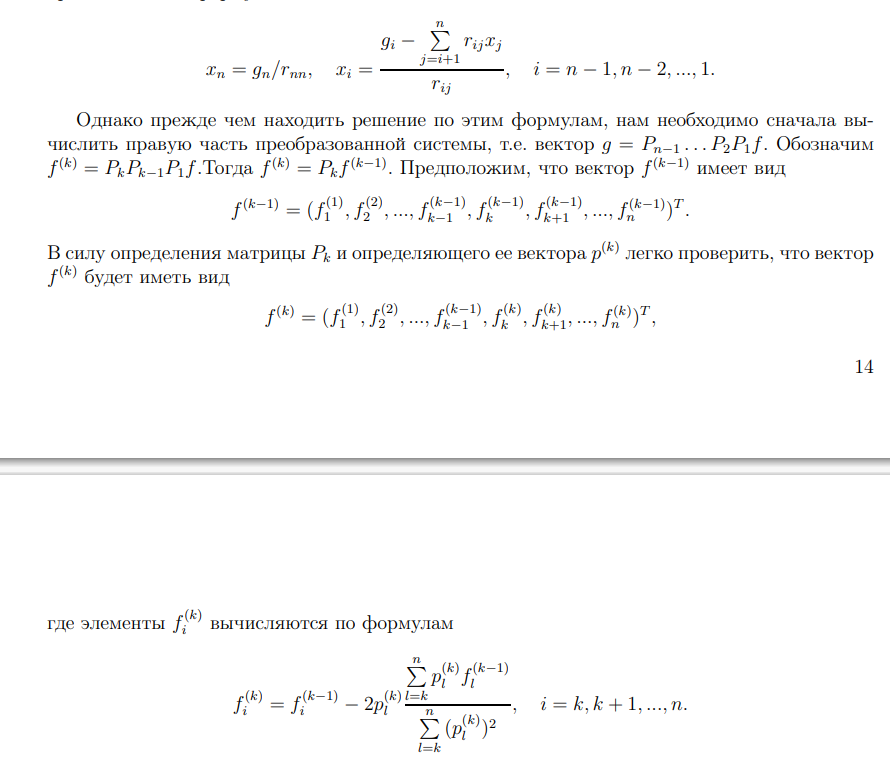
\includegraphics[width = 1\textwidth]{Screenshot_2.png}}
\end{figure}
\end{document}